%%%%%%%%%%%%%%%%%%%%%%%%%%%%%%%%%%%%%%%%%%%%%%%%%%%%%%%%%%%%%%%%%%%%%%%%%%%%%%%
%% Supporting figures distributed with the replication package.
%% Moved out of the main article to keep it within its page budget.
%% Build with: latexmk -pdf supplementary.tex
%%%%%%%%%%%%%%%%%%%%%%%%%%%%%%%%%%%%%%%%%%%%%%%%%%%%%%%%%%%%%%%%%%%%%%%%%%%%%%%
\documentclass[11pt,a4paper]{article}

\usepackage[margin=2.5cm]{geometry}
\usepackage{graphicx}
\usepackage[utf8]{inputenc}
\usepackage[hidelinks]{hyperref}

% Each figure lives with the research question that produces it.
\graphicspath{{../rq1/figures/}{../rq2/figures/}}

\renewcommand{\thefigure}{S\arabic{figure}}

\title{Supporting Figures for\\
       \emph{Simple Code, More Scrutiny:\\
       Python Proficiency and Review Effort in AI Agent and Human Pull Requests}}
\author{Chaiyong Ragkhitwetsagul, Nanthit Temkulkiat, Morakot Choetkiertikul,\\
        Ruksit Rojpaisarnkit, Raula Gaikovina Kula, and Matheus Paixao}
\date{}

\begin{document}
\maketitle

This document contains supporting figures referenced from the main article and
distributed with its replication package. They present the same underlying data as
tables that appear in the article, at a finer granularity, and are provided here so
that the article itself remains within its page budget.

\section{Per-agent proficiency by PR task type}

Figures~\ref{fig:cefr_top5_task_types} and~\ref{fig:cefr_remaining_task_types} split
each PR task type further by agent, showing the proficiency distribution of every task
type and agent combination as a separate panel.
Figure~\ref{fig:cefr_top5_task_types} covers the five task types with the most PRs, and
Figure~\ref{fig:cefr_remaining_task_types} the remaining five.
They expand the aggregated task-type breakdown given in Table~4 of the article.

A panel is left empty when the agent has no merged PR of that task type in our sample.
This is the case for build PRs by Devin and Cursor, CI PRs by Copilot and Cursor,
performance PRs by Devin, and PRs labelled \texttt{other} by Copilot and Devin.
The panels confirm that the dominance of A1 constructs holds for every agent within every
task type, and that the differences between task types are larger than the differences
between agents within a task type.

The sparsely populated panels should not be over-interpreted.
The docs panel for Cursor, for instance, consists of a single PR contributing only two
constructs, both at B1, which is why it departs from the pattern shown by the other
documentation PRs.
The PR counts behind every panel are listed in the accompanying data files.

\begin{figure}[htbp]
    \centering
    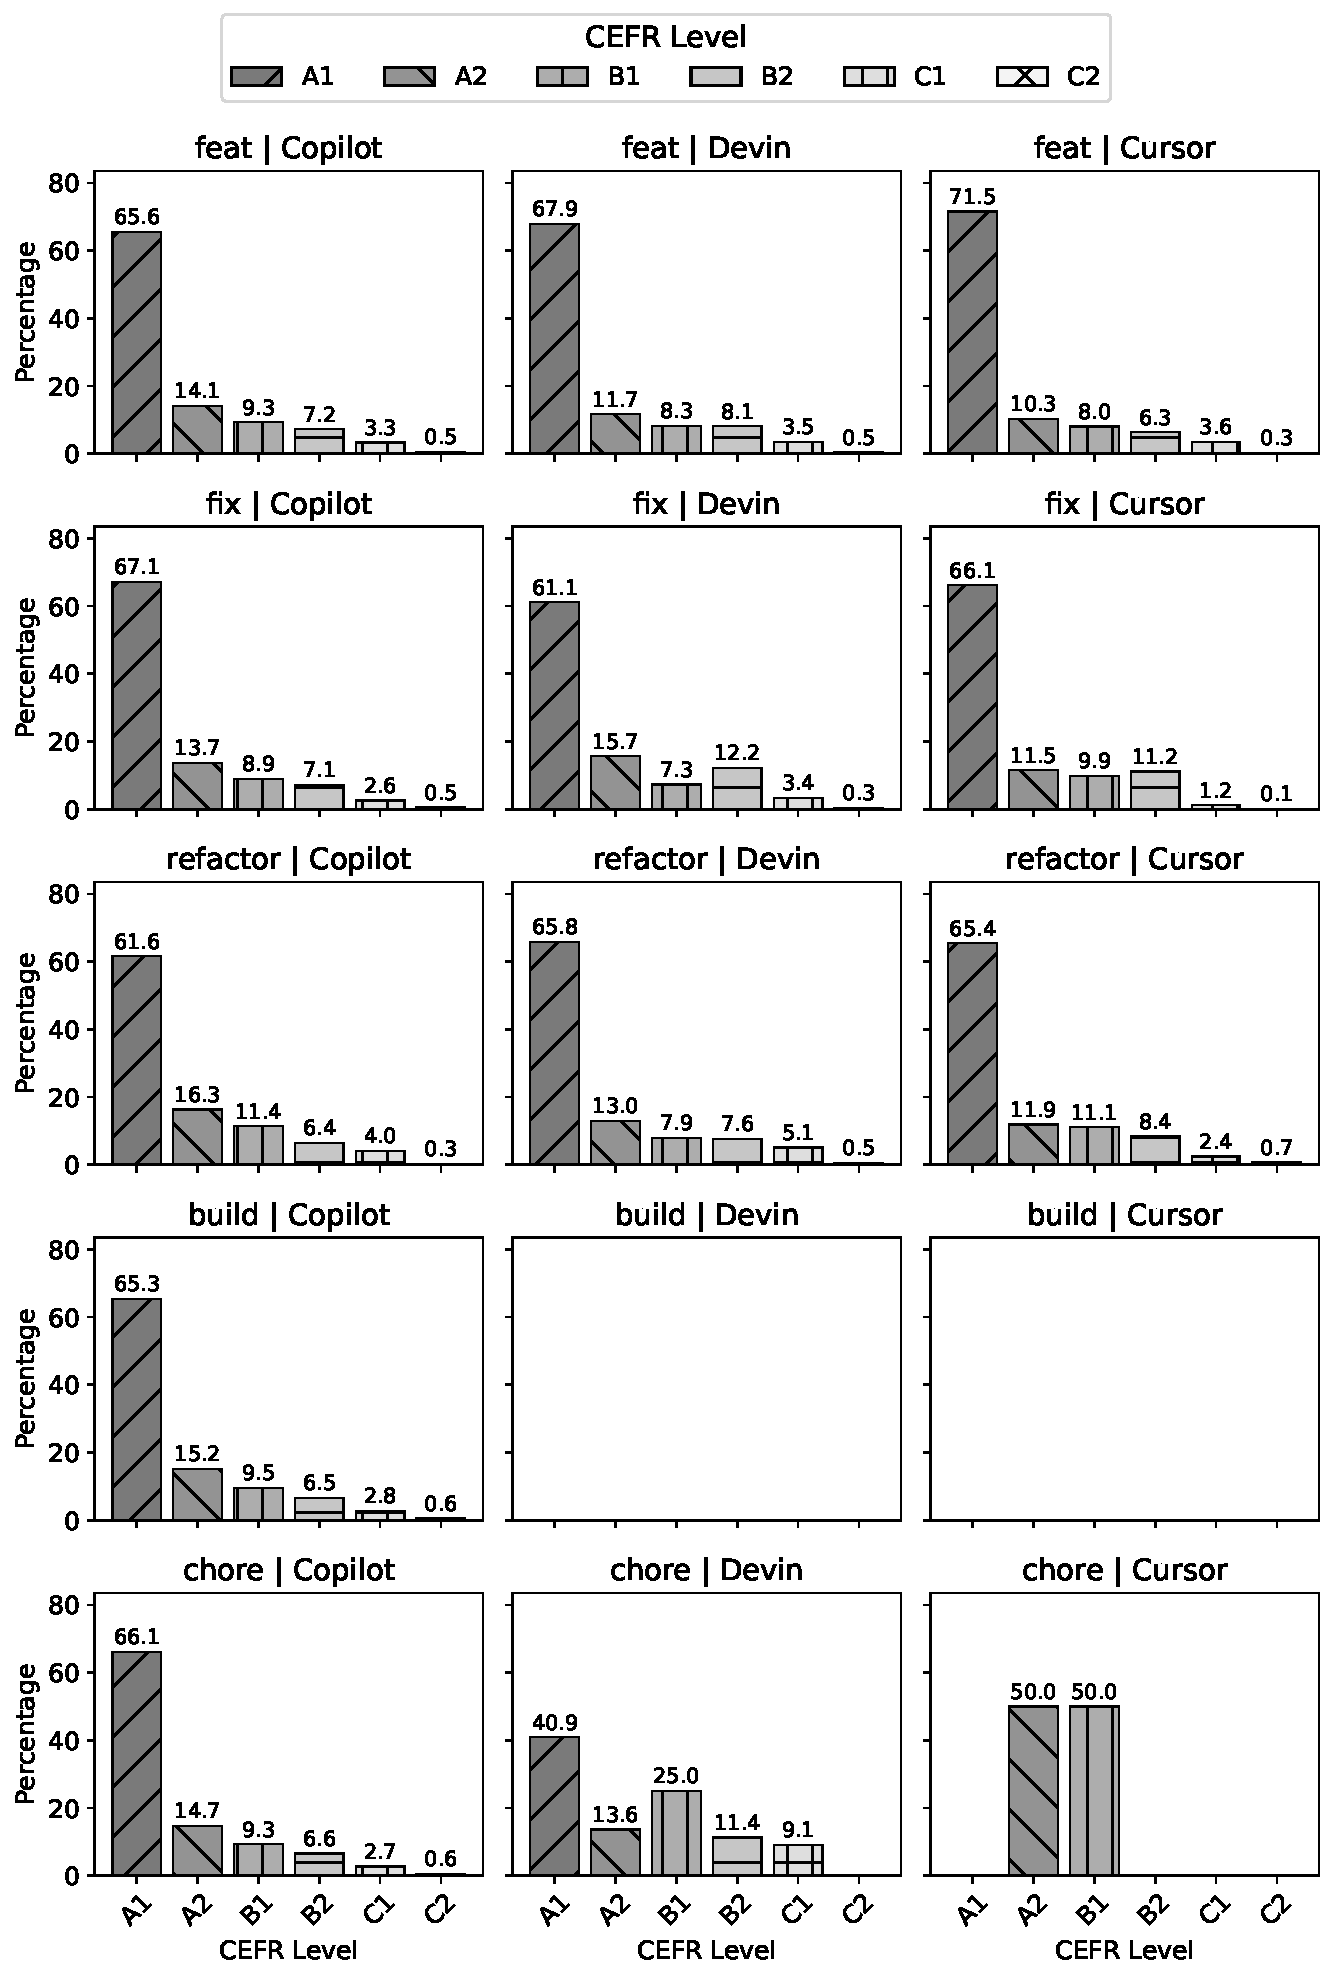
\includegraphics[width=0.9\linewidth]{cefr_top5_task_types.pdf}
    \caption{Distribution of code proficiency generated by AI agents for the 5 task types: feat, fix, refactor, build, and chore}
    \label{fig:cefr_top5_task_types}
\end{figure}

\begin{figure}[htbp]
    \centering
    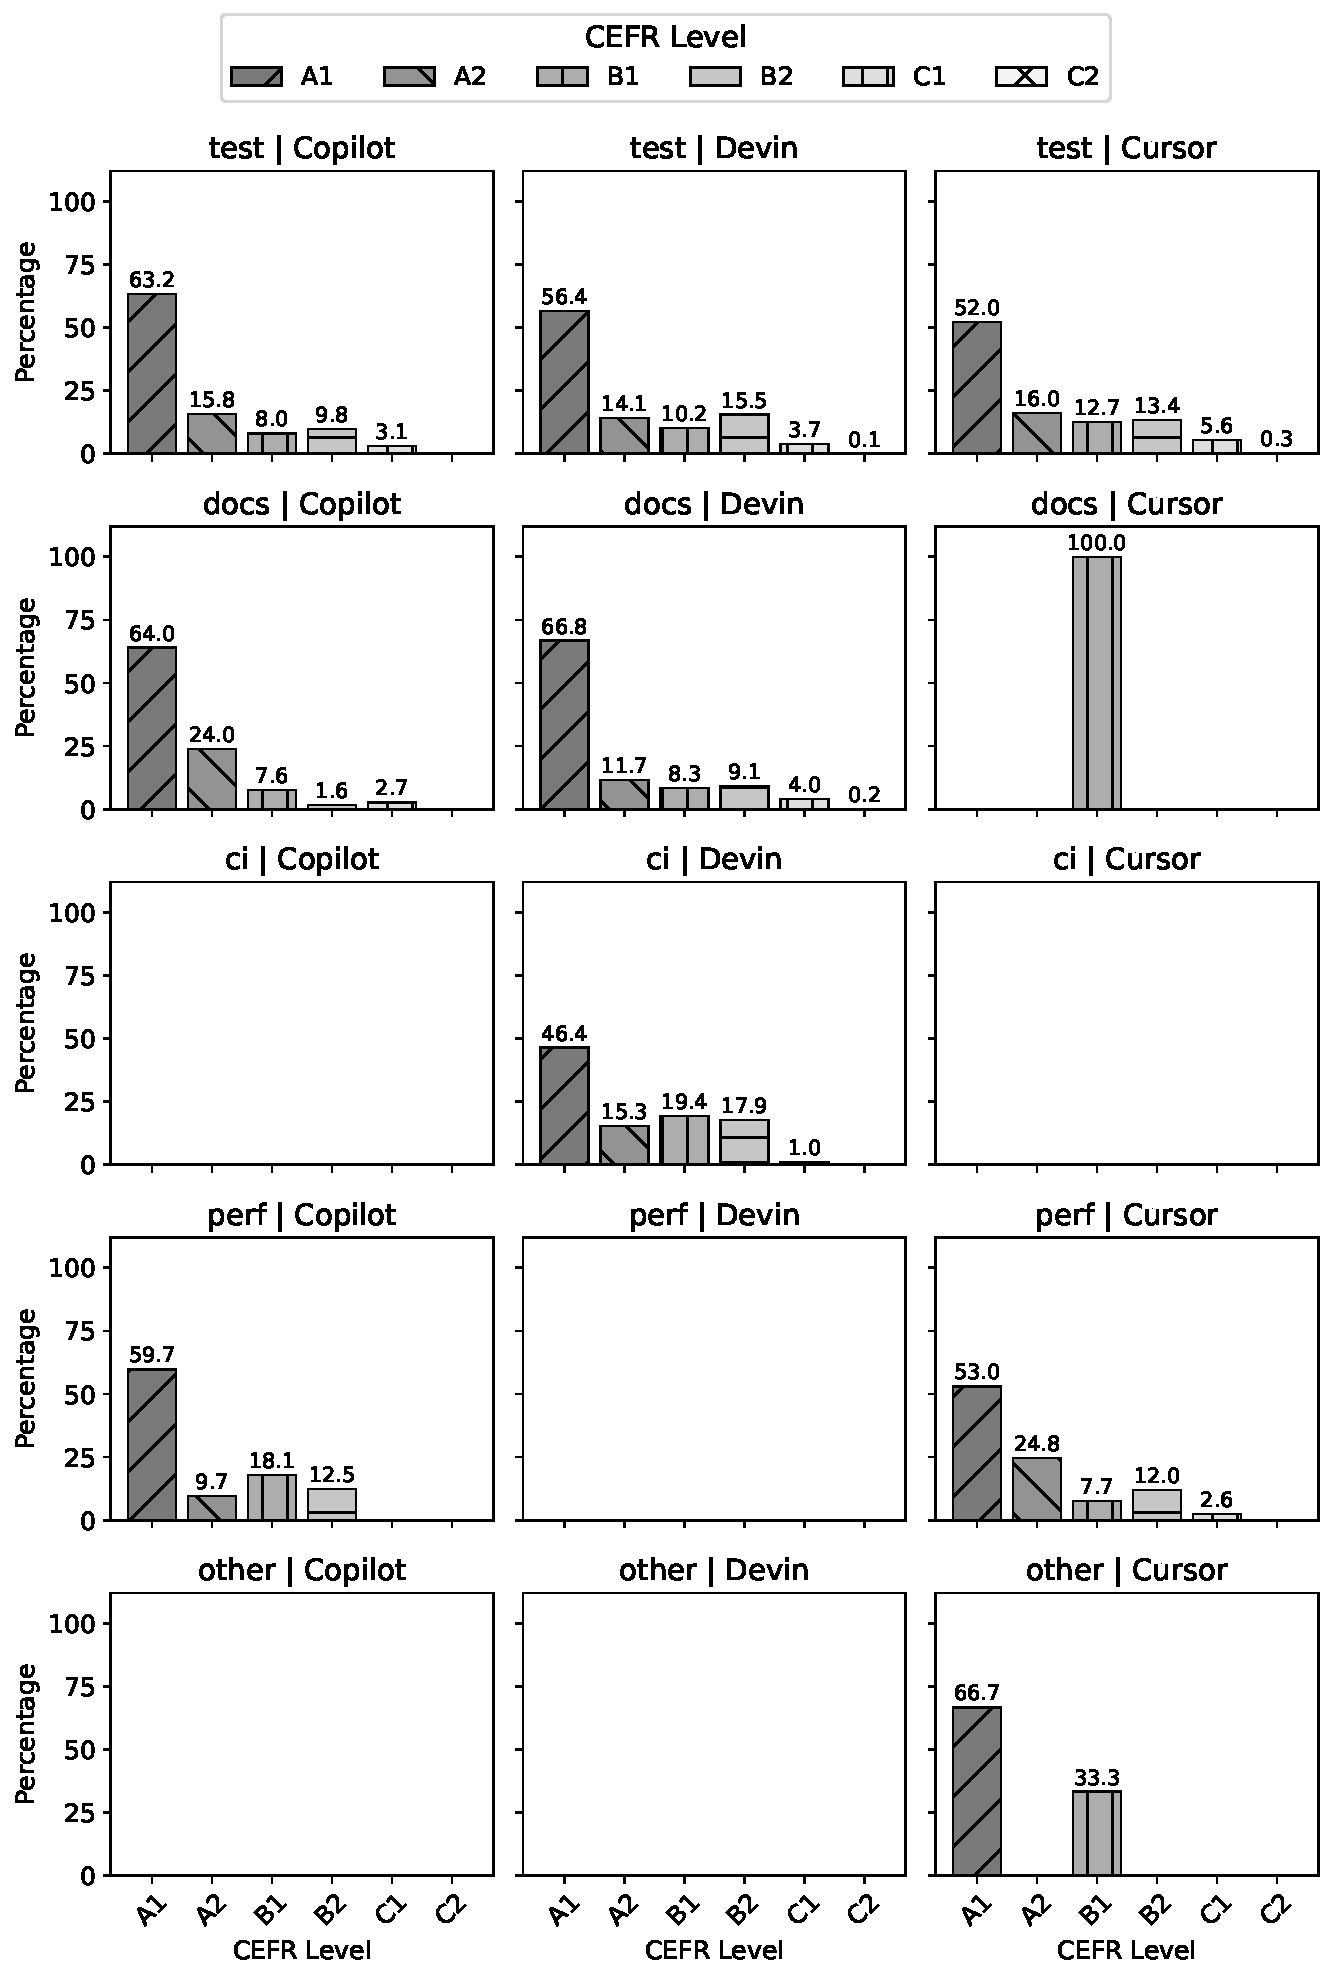
\includegraphics[width=0.9\linewidth]{cefr_remaining_task_types.pdf}
    \caption{Distribution of code proficiency generated by AI agents for the remaining task types: test, docs, ci, perf, and other}
    \label{fig:cefr_remaining_task_types}
\end{figure}

\clearpage
\section{Per-repository proficiency across the three groups}

Figure~\ref{fig:repo_paired} shows the mean ordinal CEFR score of each group in each of the
twelve repositories to which all three groups contributed code.
It accompanies the repository-paired Wilcoxon signed-rank tests reported in RQ2 of the
article.
The three groups exchange positions from one repository to the next, and no group is
systematically higher than the others, which is consistent with the tests finding no
difference for any pair.

\begin{figure}[htbp]
    \centering
    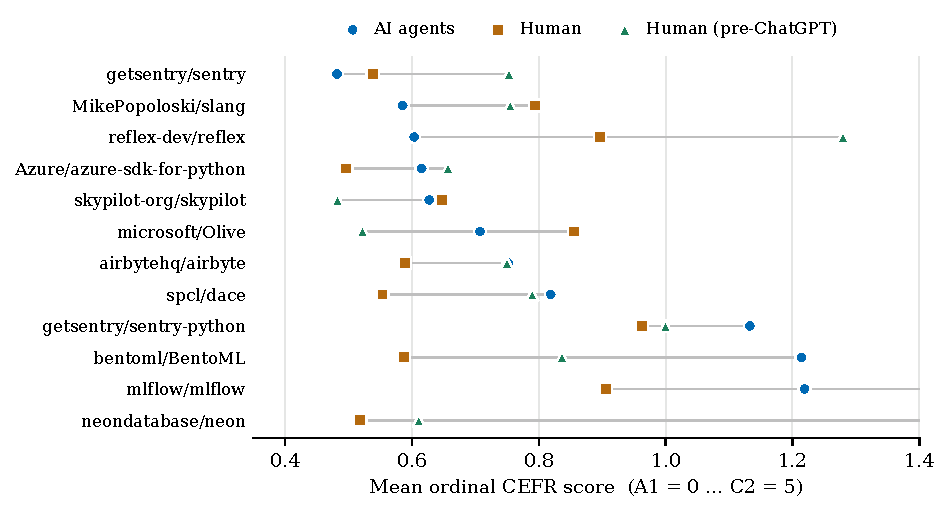
\includegraphics[width=\linewidth]{repo_paired_cefr.pdf}
    \caption{Mean ordinal CEFR score per repository for the three groups, across the twelve repositories present in all three. Repositories are ordered by the AI agents' score.}
    \label{fig:repo_paired}
\end{figure}

\end{document}
